\documentclass[../Book.Stress_regulation.tex]{subfiles}
\graphicspath{{\subfix{../images/}}}
\begin{document}

\label{Ex:SunSalutation}
\begin{figure}[htb!]
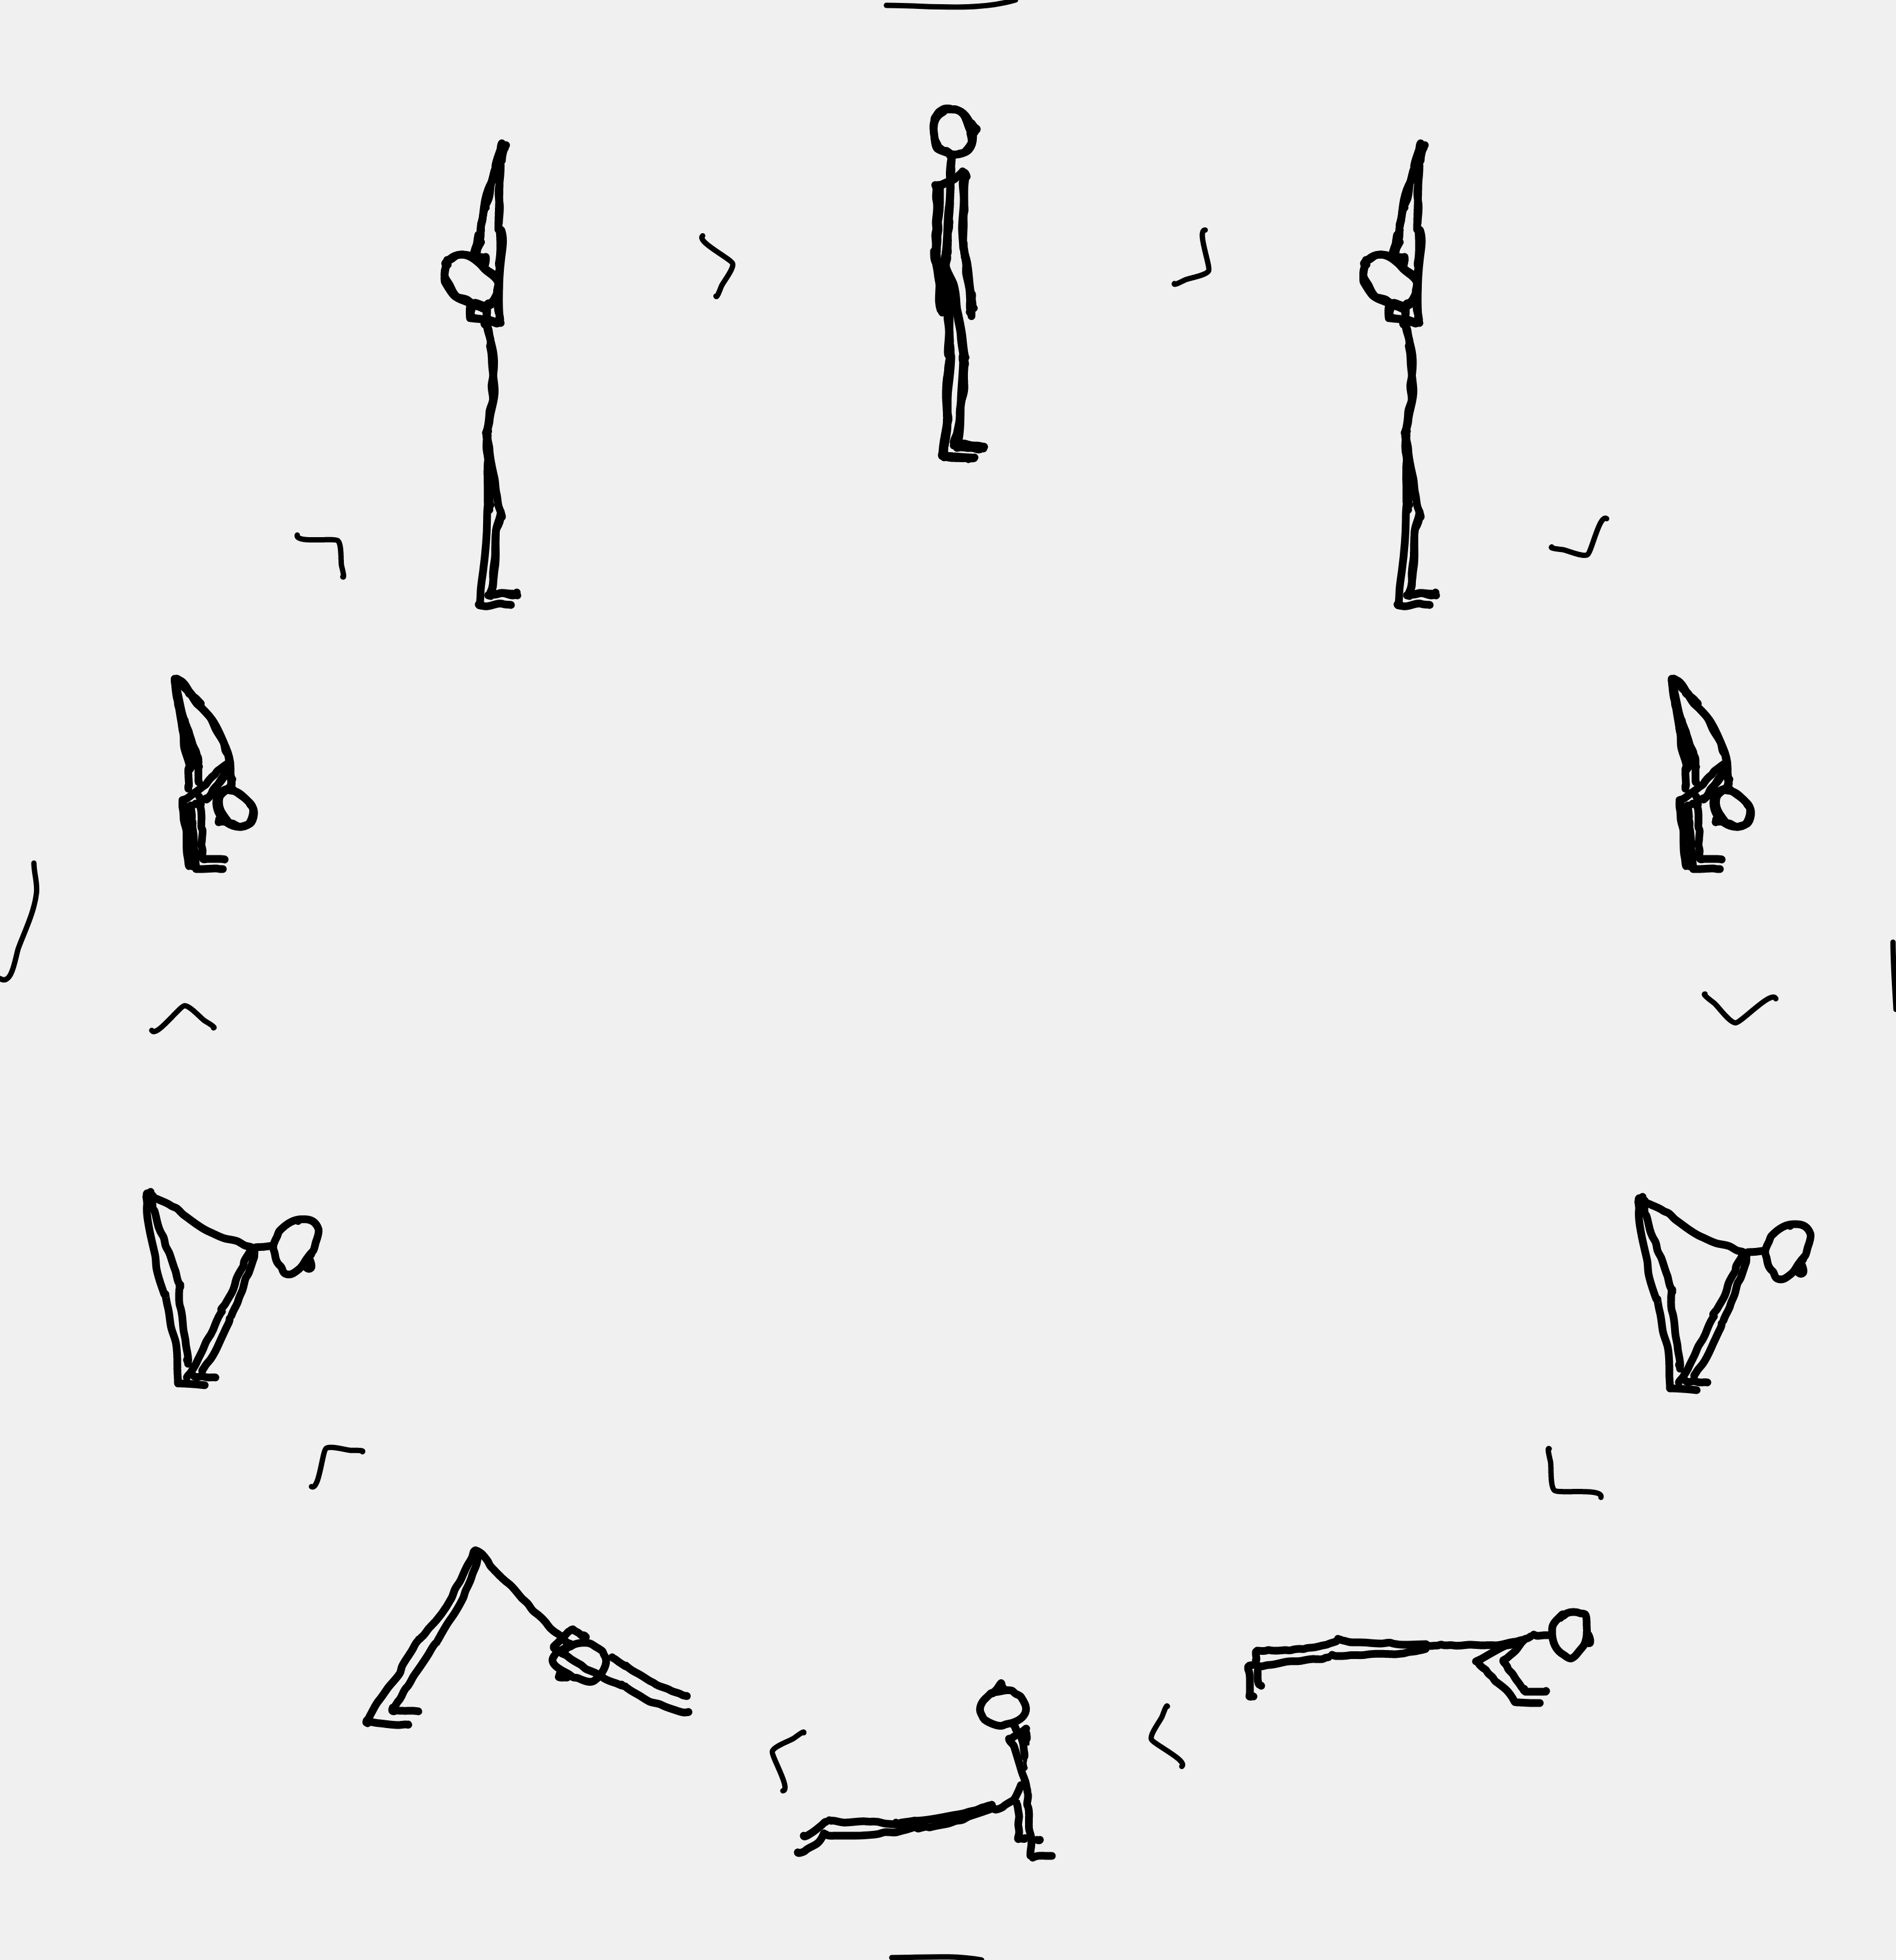
\includegraphics[width=13cm]{SunSalute}\label{sf:yoga}
\caption{Sun salutation A --- Surya Namaskar}
\end{figure}

%------------------------------------------------------------
%------------------------------------------------------------

The Sun Salutation\index{sun salutation} (sanskrit: Surya Namaskar) increases your physical strength, flexibility, your inner balance and your mental clarity.
Practiced first thing in the morning, it gets you instantaneously awake and active.
Practiced in the evening, it helps free up blocked energies.

The sun salutation is classical exercise from yoga, which consist in a fluid motion which goes through multiple positions.
The Sun Salutation stimulates all internal organs, stretches and twists the spinal cord, all the limbs and all muscle groups.
If you practice it on a regular base you will notice how it gives you strength and how you will get flooded with energy.

\begin{itemize}
\item Your breath determines the speed.
  Upon inhalation, the spine gets stretched backwards, on exhale it gets stretched forward.
  Breather calmly while executing this exercise, but consciously.
\item Make sure that you practice it in fresh air.
  Make sure that your body can move freely (no tight clothes, bare foot).
  The sun salutation is best practices before meals, otherwise your energy and your blood are going to be occupied with digestion.
\item Execute all exercises calmly and without pressure. If you are not flexible enough yet for a posture, then go as far as you are able to go, without forcing it.
  It's important that the movements are executed fluidly and consciously --- in your mind intended as a salutation to the sun.
\item In the beginning, you will probably be unable to bring your head down to your knees, or touching the ground with your palms while bending forwards.
  Keep your patience and your sense of fun. In the beginning it's enough if the tip of your fingers touch the ground.
  Your body has to first get used to the movements and with these exercises it will get more flexible and will get to move smoothly.
\end{itemize}

There are many different types of the sun salutation out there.
There is no one correct passed down tradition of yoga, but only old scripts of poses were discovered and their interpretation gave rise to the modern practice of yoga.
The sequence of the sun salutation shown in the picture above is a common version of the sun salutation, practiced in many different yoga traditions.
The sequence that I am teaching here is a version which is less straining and well suited for people of advanced age or with physical impairments, as it is easier on the body\cite{VidyaYoga}.
For me it's more important that the practice is sustainable and fun, then possible ``the correct version'' but more strenuous, and more likely to demotivate people.
Fun with the activity is an important part of practice and makes it way more likely a practice that I can sustain over time.
If you learned a different sequence of sun salutation in your yoga class, by all means  practice the one you are familiar with.

\newpage

\subsubsection{1. Mountain Pose: Stand Upright}

\begin{tabular}{p{1.4cm} p{10.1cm}}
  \raisebox{-1.1\totalheight}{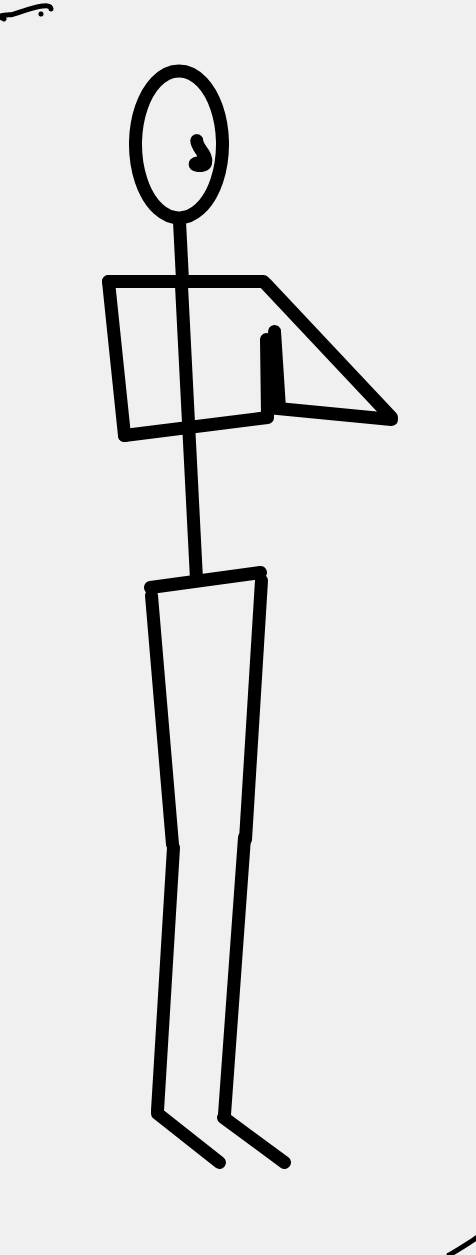
\includegraphics[width=1.6cm]{SS_Mountain}} &                                                                     
\begin{itemize}
\item Put your feet with firm pressure on the ground. Pay attention that your toes don't claw into the ground.
\item Lock your knees. By doing this, your legs will get stretched (exception: people with knee problems: leave your knees slightly bend).
\item Turn the tailbone down and forward, tense up the muscles of the pelvic floor and the sphincter of your anus. The pelvis lifts up.
\item Tense up the abs.
\item Widen and lift your chest.
\item Bend your shoulder blades backwards and lower them.
\item Feel into the posture, from the feet up the the crown.
\item Put your hands into a salutation pose and focus on the area of your heart.
\item Slightly lower your head.
\item Let your breath flow slowly and calmly, interlock your thumbs and exhale deeply.
\end{itemize}
  
\end{tabular}

\subsubsection{2. Opening Up: Lead your Hands up in Front of your Head}

\begin{tabular}{p{1.3cm} p{10.2cm}}
     \raisebox{-1.05\totalheight}{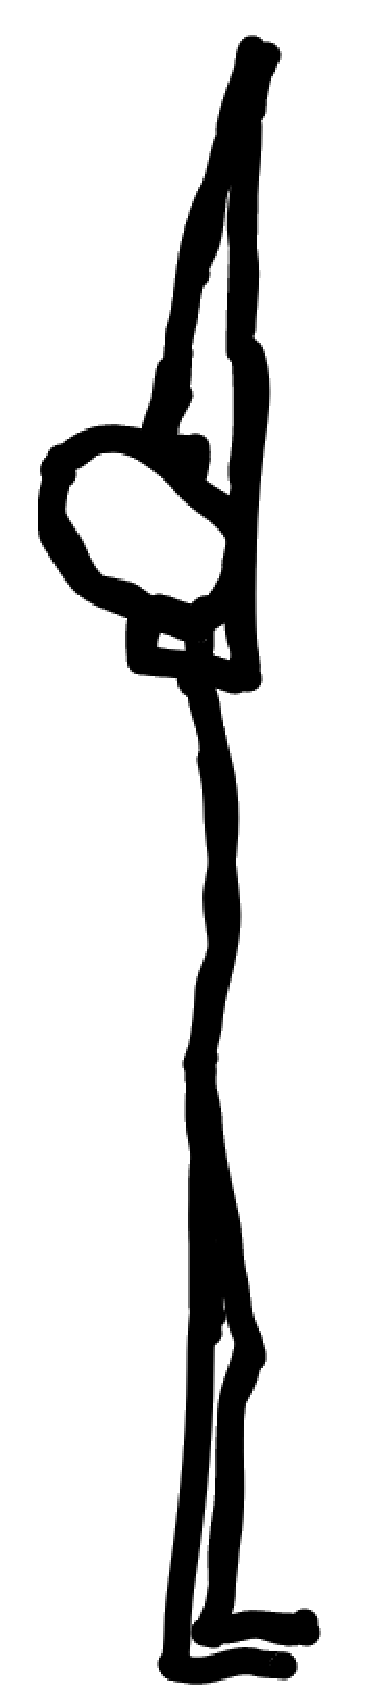
\includegraphics[width=1.35cm]{SS_Opening}}
& 
\begin{itemize}
\item Inhale deeply.
\item Keep your thumbs in the interlocked position, but open the hands and stretch the locked elbows as far back as possible, until the hands are above the crown of your head. Important: Keep your hip stable.
\item The palms of your hands point upwards and the fingers are flexed backwards.
\item Stretch your thoracic spine and lift your sternum forward and upwards.
\item By doing so, achieve a slight backwards bend of the upper back, with which you achieve a widening of the width and height of your chest.
\item Pay attention in the posture, that the hip stays stable. It should stay unmoved in the axis of the legs.
\item Focus on the area of your forehead.
\end{itemize}  
\end{tabular}


\subsubsection{3. Bend Forward: Touch the Floor with your Hands}


\begin{tabular}{p{1.3cm} p{10.3cm} }
  \raisebox{-1.1\totalheight}{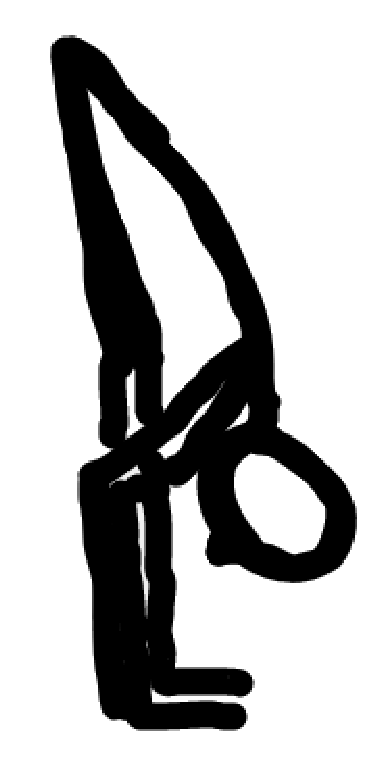
\includegraphics[width=1.3cm]{SS_ForwardBend}}
  &
\begin{itemize}
\item Exhale.
\item Lead your arms in direction of the floor, leading with the tips of your fingers. Start exhaling.
  On the height of your chest, the palms start pointing towards the ground. 
\item Start bending forward, put your hands next to your body (Variant: grip your big toes with your thumb  and index, the thumbs are on the toes).
\end{itemize}
\end{tabular}
\noindent \vspace{-5mm}
\begin{itemize}
\item Push with your hip (backside) slightly upwards and backwards. This gives a stretch in the legs and the back stays relaxed.
  If you can't reach the floor with your legs locked and straight, then bend your knees but still push with your hips towards the ceiling.
\item Try to touch with your belly the thighs and let your head hang.
\item Bend your chin slightly towards the throat.
\item Keep pushing your hips towards the ceiling.
\item Put you focus on the abdomen and exhale completely.  
\end{itemize}
  



\subsubsection{4. Warrior Pose: Put your Left Leg Backwards in the Emptiness before your Inhale}
\begin{tabular}{p{5.5cm} p{6cm} }
  \raisebox{-1.1\totalheight}{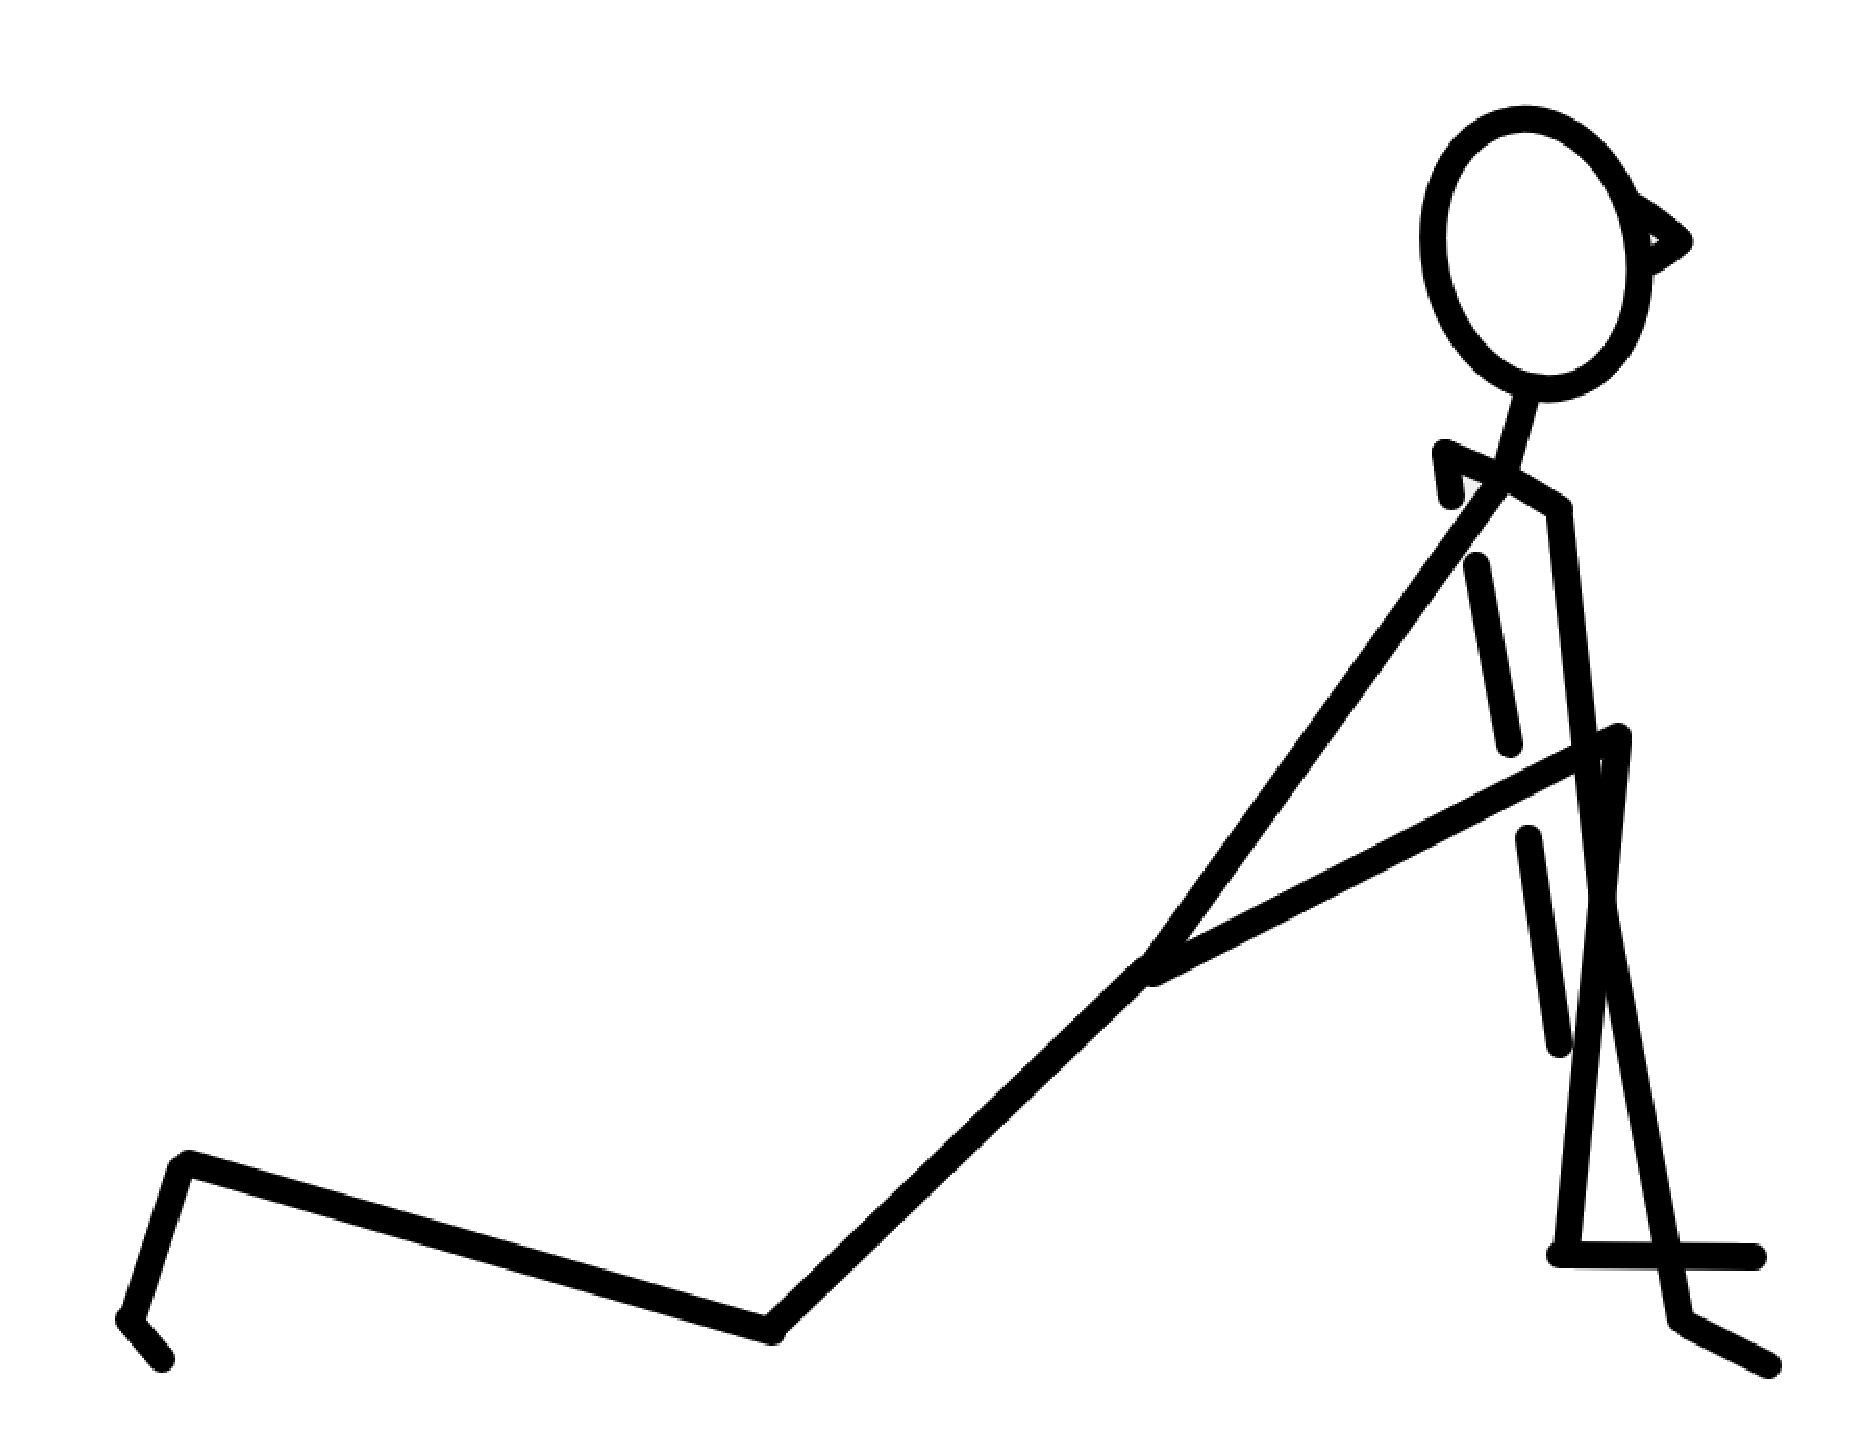
\includegraphics[width=5.5cm]{SS_Warrior}}
  &
\begin{itemize}
\item Your left knee stands on the ground, the foot stands on the upward flexed (or later on on the stretched out) toes.
\item Bend your right knee above your right foot.
\item Rotate the pelvis forward and downward.
\item Simultaneously urge with your tail bone downward and forward.
\item While inhaling, erect your torso.
\item Lift your chest and reach with it forward. Lead your arms downwards, along your body, in direction of your feet.
  Eventually you can touch the floor with the tip of your fingers.
\item Direct your gaze forwards.
\item Focus and center on the area of your heart.    
\end{itemize}
\end{tabular}



\subsubsection{5. Inclined Plane: Stretch your Right Bend Leg Backwards}
\begin{tabular}{p{5.5cm} p{6cm} }
  \raisebox{-1.1\totalheight}{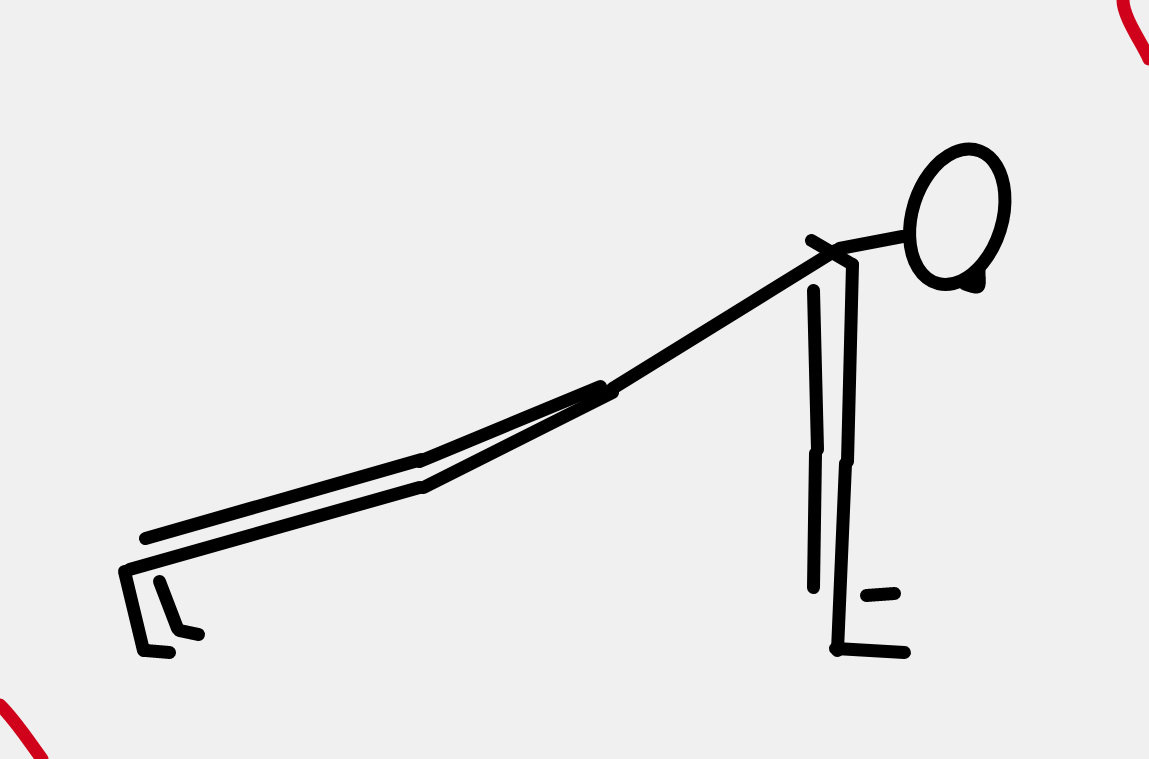
\includegraphics[width=5.5cm]{SS_Plank}}
  &

\begin{itemize}
\item Hold your breath.
\item Stretch your body, until it is in one straight line.
\item Put your feet on your toes, which are bend towards the center (towards your belly).
\item Your arms are holding your body straight, they should be in a right angle with respect to the floor.
\item Pay attention that your hip is in one straight line with the legs and the torso.
  Your whole body is in one straight line, from your head to your feet (don't let your head fall).
\item The soles of your feet lift off the floor, the toes stay in place.
\end{itemize}
\end{tabular}

\subsubsection{6. Downward Dog: Lift your Buttocks Upward}

    
\begin{itemize}
\item Shift your weight.
\item At the same time, press your heels into the ground.
\item Push your hips backwards and upwards and push your buttocks towards the ceiling.
\item Exhale and press your hands towards the floor. The ball of the thumb and the tips of your finger should be in solid contact with the floor.
  Pay attention that the bones of the middle of your hand (metacarpus) aren't locked.
\item (Over time!), the feet gain complete contact with the floor.
  If this isn't possible yet, try to get them as much as possible into contact with the floor.
\item Lock your arms and your legs.
\item Bend your upper back slightly backwards, the chest approaches the floor while exhaling.
  If you are having difficulties with the exercise, you can slightly bend the knees
  (while still pushing the buttocks towards the ceiling), in order to better achieve the opening of the chest.
\end{itemize}
\vspace{-5.5mm}\hspace{-3.5mm}

\noindent\begin{tabular}{p{6cm} p{5.5cm}}
\begin{itemize}
\item The head should be held in the prolongation of the spine.
\item Focus on the middle of your body.
\item  Exhale very deeply, contract in the meanwhile your abdominal wall towards the spine.
\end{itemize}
&
\raisebox{-1.1\totalheight}{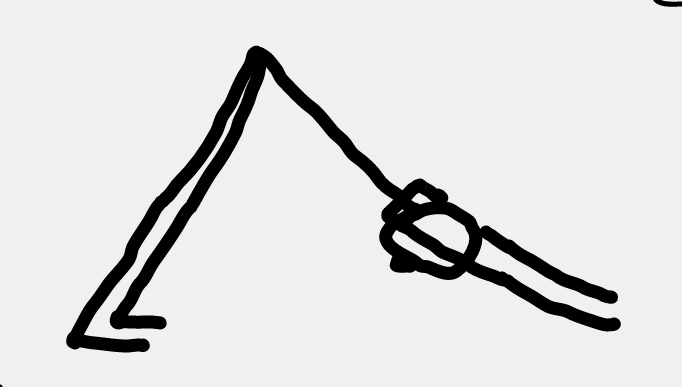
\includegraphics[width=5.5cm]{SS_DownwardDog}}
\end{tabular}

\subsubsection{7. Eight fold Prostration: Lower your Body to the Floor}

\noindent
\begin{tabular}{p{6cm} p{5.5cm}}
 \raisebox{-1.1\totalheight}{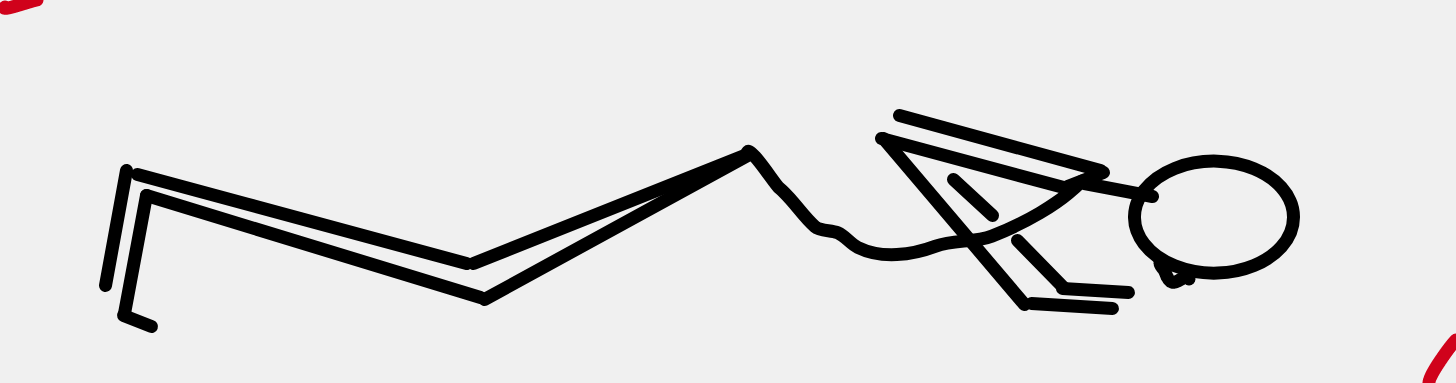
\includegraphics[width=6cm]{SS_Prostrate}}
\begin{itemize}
\item This posture is called eight fold prostration, because only eight parts of your body touch the floor: forehead, chest, knees, both legs and both hands.
\item Lower your body evenly to the ground, with the above mentioned parts of your body.
\item Focus your attention on the region of your belly and your chest and the forehead.
\end{itemize}
\end{tabular}
          

\subsubsection{8. Cobra: Lower your Pubic Bone to the Floor}
\begin{itemize}
\item Inhale deeply.
\item Push with your tail bone downwards and forwards to the middle of the pelvic floor and thereby slightly tense up the muscles of your pelvic floor.
\item Lower the back your your feet to the floor.
\item Push your whole body forward and put your upper back into a backwards bend upon inhale.
\item Relax your buttocks muscles.
\item The force to erect your upper torso comes from the muscles of the upper back.
\item Your elbows push backwards and are close to your body, your shoulders point outwards and downwards.
  Your shoulder blades approach each other.
\end{itemize}
\vspace{-5.5mm}\hspace{-3.5mm}
\noindent\begin{tabular}{p{6cm} p{5.5cm}}
\begin{itemize}
\item Your elbows push backwards and are close to your body, your shoulders point outwards and downwards.
  Your shoulder blades approach each other.
\item Open and widen your chest and look upwards.
\item Focus your attention on the region of your heart.
\end{itemize}
&
\raisebox{-1.1\totalheight}{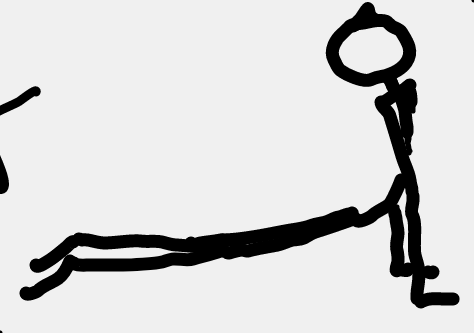
\includegraphics[width=5.8cm]{SS_Cobra}}
\end{tabular}

\subsubsection{9. Downward Dog: Lift your Buttocks Backwards and Upward}
\begin{itemize}
\item With your lungs full of air, contract the muscles of the pelvic floor.
\item Exhale and press your hands towards the floor. The ball of the thumb and the tips of your finger should be in solid contact with the floor.
\item (Over time!), the feet gain complete contact with the floor.
\item Lock your arms and your legs.
\item Bend your upper back slightly backwards, the chest approaches the floor while exhaling.
  If you are having difficulties with the exercise, you can slightly bend the knees.
\end{itemize}
\vspace{-5.5mm}\hspace{-3.5mm}
\noindent\begin{tabular}{p{6cm} p{5.5cm}}
\begin{itemize}
\item The head should be held in the prolongation of the spine.
\item Focus on your middle.
\item  Exhale very deeply, contract in the meanwhile your abdominal wall towards the spine.
\end{itemize}
&
\raisebox{-1.1\totalheight}{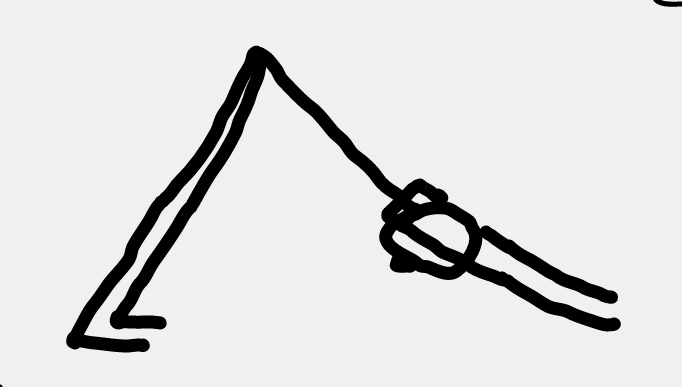
\includegraphics[width=5.5cm]{SS_DownwardDog}}
\end{tabular}
          
\subsubsection{10. Warrior Pose: Put your Left Forward}
\begin{tabular}{p{3cm} p{8.6cm} }
  \raisebox{-1.1\totalheight}{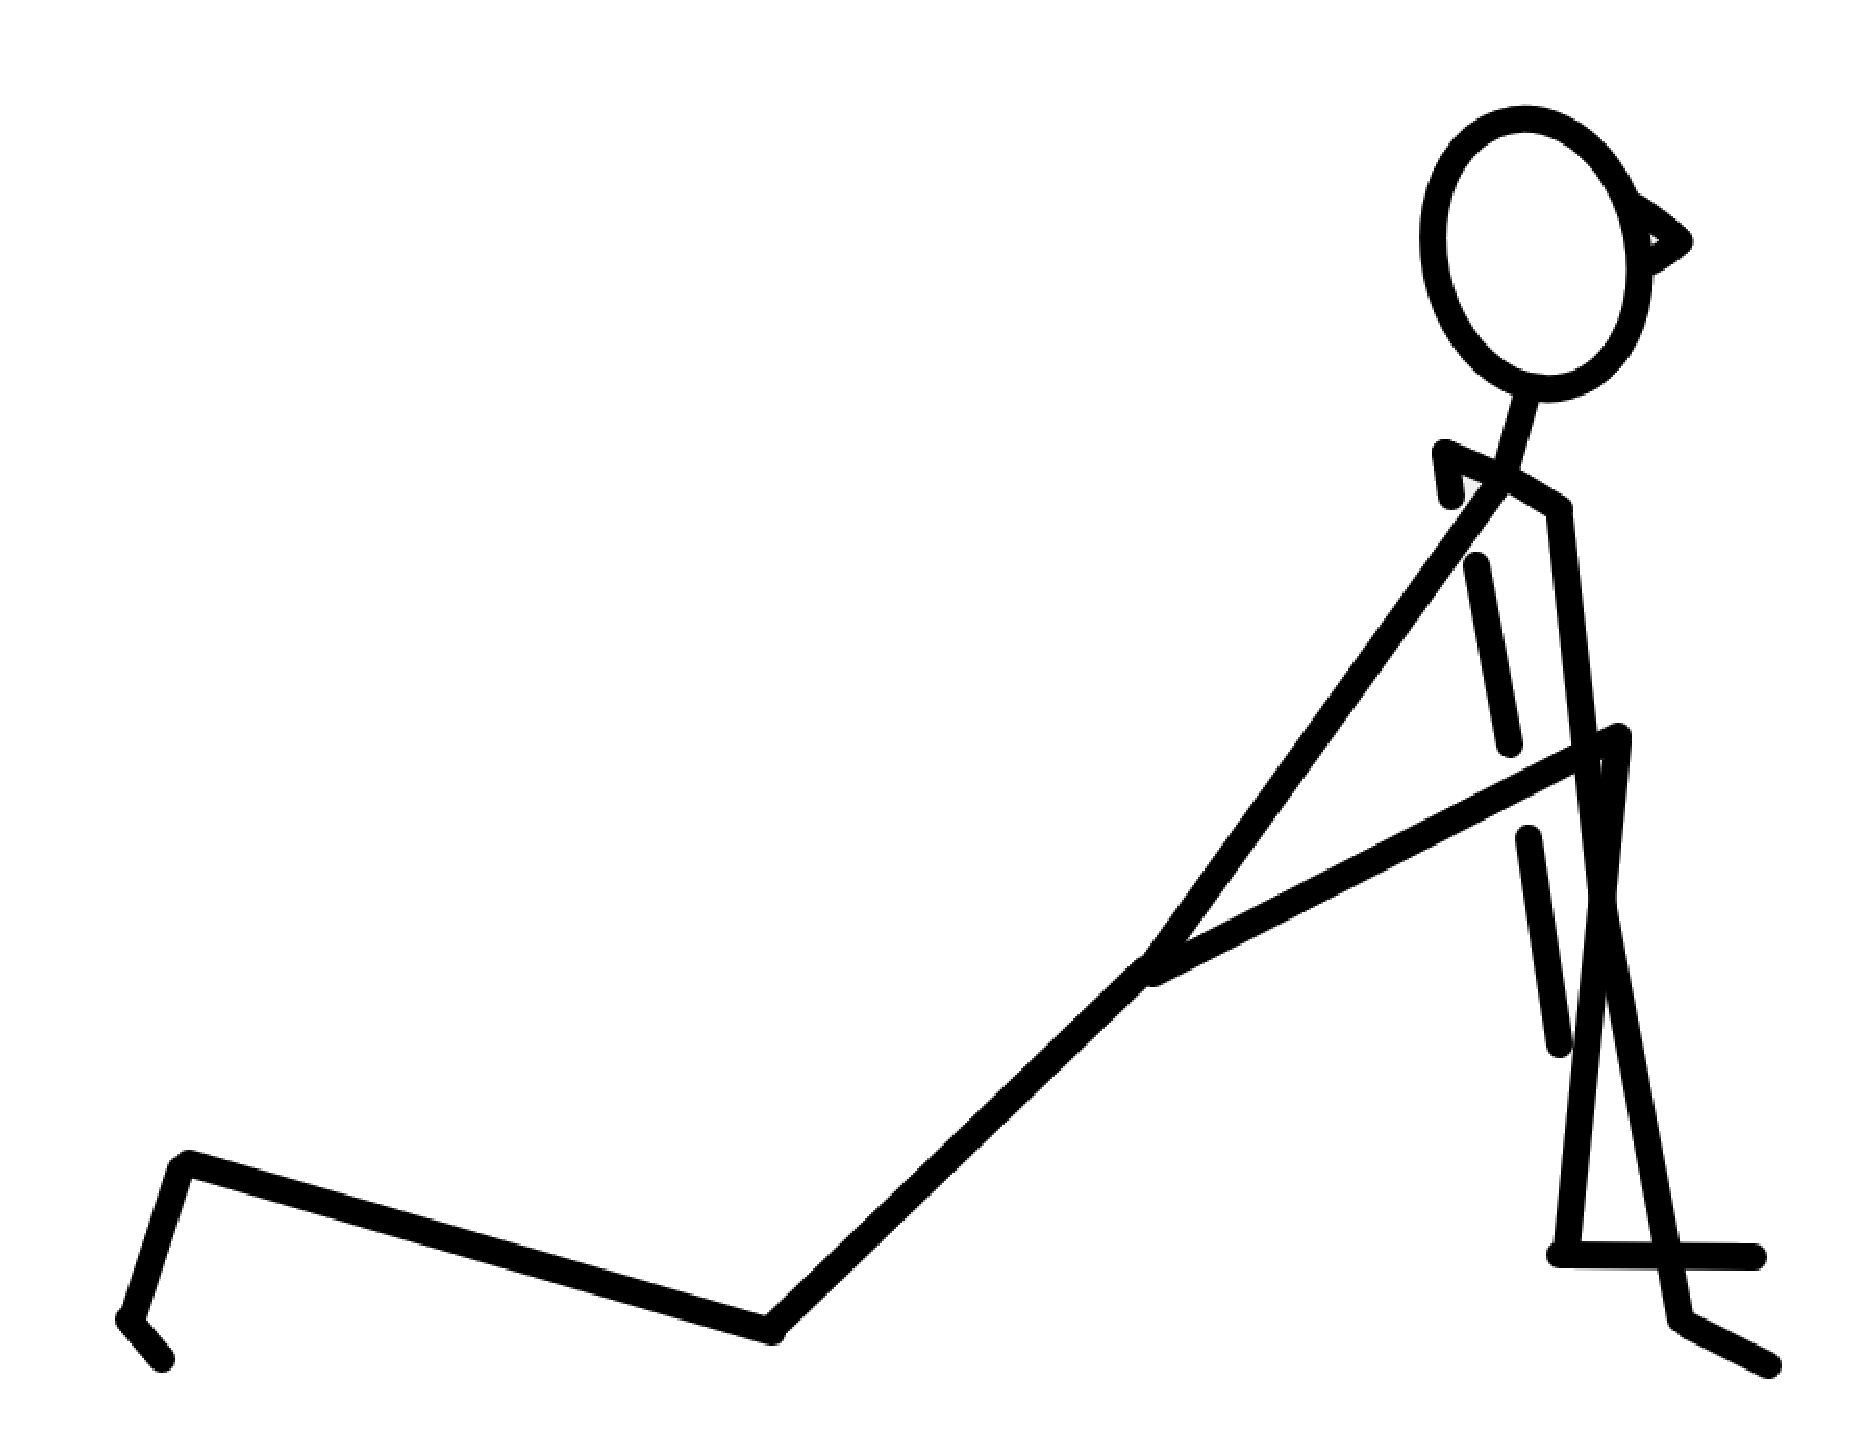
\includegraphics[width=3cm]{SS_Warrior}}
  &

\begin{itemize}
\item In the emptiness of your lungs, between two breaths, put your left foot forward between your hands.
  \item Bend your left knee above your left foot.
\item Your right knee stands on the ground, the foot stands on the upward flexed toes.
\item Rotate the pelvis forward and downward.
\item Simultaneously urge with your tail bone downward and forward.
\item While inhaling, erect your torso.
\item Lift your chest and reach with it forward. 
\item Direct your gaze straight forward.
\item Focus and center on the area of your heart.    
\end{itemize}

\end{tabular}


\subsubsection{11. Bend Forward: Bring your Right Foot next to your Left Foot}
\begin{tabular}{p{9.7cm} p{1.8cm}}

\begin{itemize}
\item Place your hands next to your feet.
\item Stretch and lock your legs.
\item Push with your hip slightly upwards and backwards. This gives a stretch in the legs and the back stays straight and relaxed.
  If you can't reach the floor with your legs locked and straight, then bend your knees but still push with your hips towards the ceiling.
\item Try to touch with your belly the thighs and let your head hang.
\item Put you focus on the abdomen.
\item Exhale completely.
\end{itemize}
    &
    \raisebox{-1.2\totalheight}{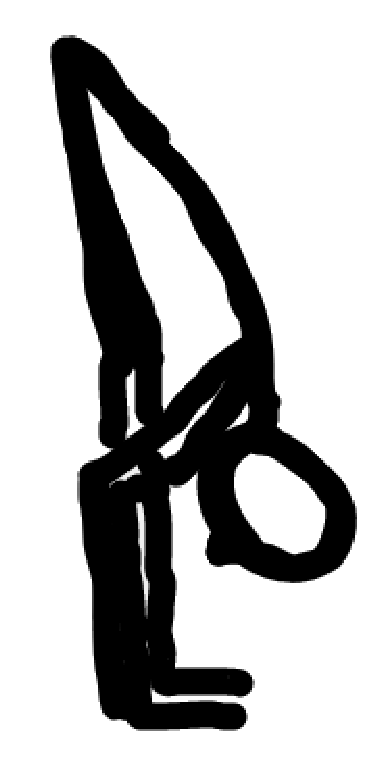
\includegraphics[width=1.8cm]{SS_ForwardBend}}
  
\end{tabular}

\subsubsection{12. Opening Up: Lead your Hands up in Front of your Head}

\begin{tabular}{p{9.7cm} p{1.8cm}}
  
\begin{itemize}
\item Inhale deeply again.
\item Tense up the muscles of your buttocks, detach your hands from the floor and join your hands with the palms.
\item Slowly erect your torso, Your hands raise up in a smooth motion in front of your head during a deep inhale.
  Interlock your thumbs in the meanwhile.
\item Open the hands and stretch the locked elbows as far back as possible, until the hands are above the crown of your head. Keep your hip totally stable.
\item The palms of your hands point upwards and the fingers are flexed backwards.
\item Stretch your thoracic spine and lift your sternum forward and upwards.
\item By doing so, achieve a slight backwards bend of the upper back, with which you achieve a widening of the width and height of your chest.
\item Pay attention in the posture, that the hip stays stable. It should stay unmoved in the axis of the legs.
\item Focus on the area of your forehead.
\end{itemize}
  &
    \raisebox{-1.2\totalheight}{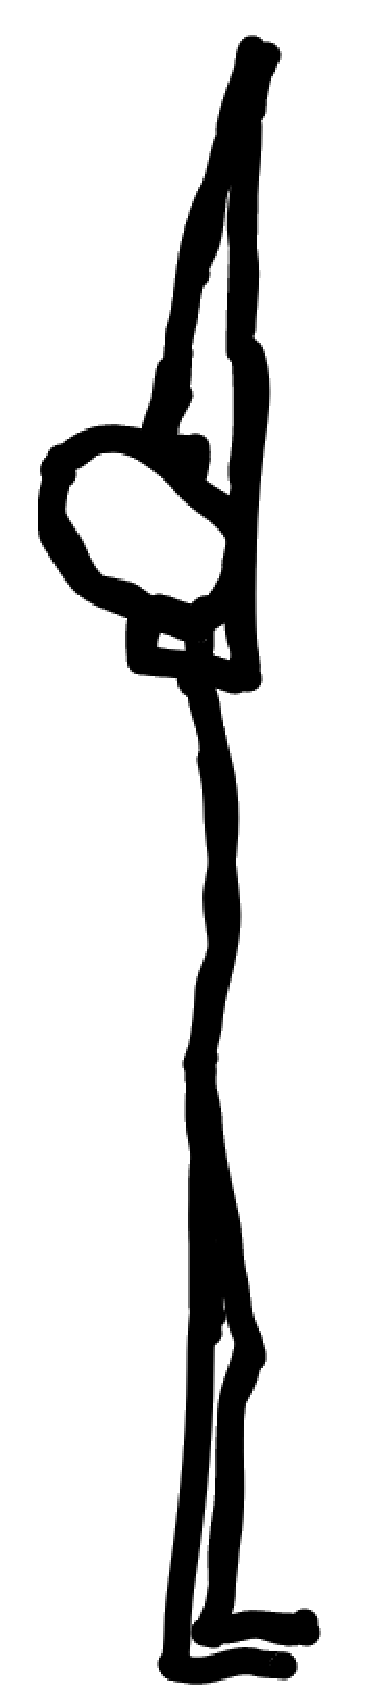
\includegraphics[width=1.3cm]{SS_Opening}}
  
\end{tabular}

If you want to repeat the sequence, just continue straight into the bending forward pose.
Take this time for the warrior pose (one leg backwards) first the right leg.
After the dog pose, take this time also the right leg forward.

\subsubsection{Termination}

\begin{itemize}
\item Upon exhale, lead your hands in front of your sternum.
\item Focus your attention on the region of your heart.
\item Now lower your arms.
\item Stay a moment in this pose and feel the effects on your body.
\end{itemize}

\subsubsection{If you want to make Multiple Repetitions}

Stop the sun salutation after the cycle in which you put first your right leg backwards with these two poses.
After that start all over again for two more repetitions, once with your left leg going backwards, then the second one with your right leg going backwards.

To be clear on that point: you could think that after the described twelve poses one repetition is terminated.
In my understanding a repetition is only terminated, when once my left foot goes backwards first and then my right foot the second time round.
For me, that means being balanced.

\end{document}